% 需要的宏包：amsmath, amssymb, tikz, array

\begin{center}
    {\Large \textbf{河北工程大学 2023$\sim$2024 学年第二学期期末考试试卷（A）卷}}
\end{center}

\setcounter{section}{0}


\section{选择题（每题 2 分，共 20 分）}

\begin{enumerate}
    \item 下面句子中哪个是命题（\quad）
    \choicemid{我正在说谎话。}{你有铅笔么？}{请不要讲话！}{2030 年我会升职加薪。}

    \item 公式 $((\forall y\neg G(y)\land \forall xF(x))\land \exists yG(y))\to \forall xF(x)$ 的类型为（\quad）
    \choicemid{永真式}{永假式}{非永真式的可满足式}{不可判定类型}

    \item 已知 $A=\{1,2,3\}$，$R_1,R_2,R_3$ 是 $A$ 上的关系，以下说法错误的是（\quad）
    \choicemid{$R_1=\{\langle 1,1\rangle,\langle 2,2\rangle\}$ 不是自反的}{$R_1=\{\langle 1,1\rangle,\langle 2,2\rangle\}$ 不是反自反的}{$R_2=\{\langle 1,1\rangle,\langle 2,2\rangle,\langle 3,3\rangle,\langle 1,2\rangle\}$ 是自反的}{$R_3=\{\langle 1,3\rangle\}$ 不是反自反的}

    \item 公式 $(p\to \neg q)\to r$ 的主合取范式为（\quad）
    \choicemid{$M_0\land M_2\land M_4$}{$M_1\land M_2\land M_4\land M_6$}{$M_0\land M_3$}{$M_1\land M_3\land M_5\land M_6\land M_7$}

    \item 下面哪个等值式是错误的（\quad）
    \choicemid{$\forall x(A(x)\land B(x))\Leftrightarrow \forall xA(x)\land \forall xB(x)$}{$\exists x(A(x)\lor B(x))\Leftrightarrow \exists xA(x)\lor \exists xB(x)$}{$\forall x(A(x)\lor B(x))\Leftrightarrow \forall xA(x)\lor \forall xB(x)$}{$\exists x(B\to A(x))\Leftrightarrow B\to \exists xA(x)$}

    \item 以下哪个是欧拉图（\quad）
    \choicelow{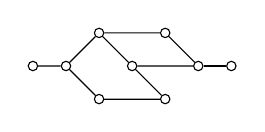
\begin{tikzpicture}[baseline=-0.5ex,scale=0.42,every node/.style={circle,draw,inner sep=1.2pt}]
            \node (a) at (0,0) {};
            \node (b) at (1,0) {};
            \node (c) at (2,1) {};
            \node (d) at (3,0) {};
            \node (e) at (2,-1) {};
            \node (f) at (4,1) {};
            \node (g) at (5,0) {};
            \node (h) at (4,-1) {};
            \node (i) at (6,0) {};
            \draw (a)--(b)--(c)--(d)--(h)--(e)--(b);
            \draw (c)--(f)--(g)--(d);
            \draw (e)--(h);
            \draw (g)--(i);
        \end{tikzpicture}}{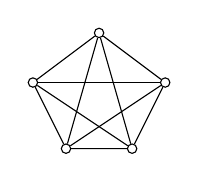
\begin{tikzpicture}[baseline=-0.5ex,scale=0.42,every node/.style={circle,draw,inner sep=1.2pt}]
            \node (a) at (0,0) {};
            \node (b) at (1,-2) {};
            \node (c) at (3,-2) {};
            \node (d) at (4,0) {};
            \node (e) at (2,1.5) {};
            \draw (a)--(b)--(c)--(d)--(e)--(a);
            \draw (a)--(c);
            \draw (a)--(d);
            \draw (b)--(d);
            \draw (b)--(e);
            \draw (c)--(e);
        \end{tikzpicture}}{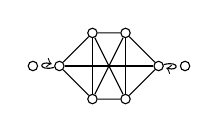
\begin{tikzpicture}[baseline=-0.5ex,scale=0.42,every node/.style={circle,draw,inner sep=1.2pt}]
            \node (a) at (0,0) {};
            \node (b) at (1,1) {};
            \node (c) at (2,1) {};
            \node (d) at (3,0) {};
            \node (e) at (2,-1) {};
            \node (f) at (1,-1) {};
            \node (l) at (-0.8,0) {};
            \node (r) at (3.8,0) {};
            \draw (a)--(b)--(c)--(d)--(e)--(f)--(a);
            \draw (a)--(d);
            \draw (b)--(e);
            \draw (c)--(f);
            \draw (b)--(f);
            \draw (c)--(e);
            \draw (a) edge[loop left] (a);
            \draw (d) edge[loop right] (d);
        \end{tikzpicture}}{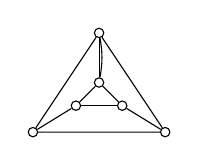
\begin{tikzpicture}[baseline=-0.5ex,scale=0.42,every node/.style={circle,draw,inner sep=1.2pt}]
            \node (a) at (0,0) {};
            \node (b) at (4,0) {};
            \node (c) at (2,3) {};
            \node (d) at (1.3,0.8) {};
            \node (e) at (2.7,0.8) {};
            \node (f) at (2,1.5) {};
            \draw (a)--(b)--(c)--(a);
            \draw (a)--(d)--(f)--(e)--(b);
            \draw (d)--(e);
            \draw (c)--(f);
            \draw (c) edge[bend left=10] (f);
        \end{tikzpicture}}

    \item 小明此刻说：“如果我不在打网球，那么我就在看网球比赛；如果我不在看网球比赛，那么我就在看网球杂志。”假如小明不能同时做两件以上的事，那么他此刻在做什么？（\quad）
    \choicelow{在打网球}{在看网球比赛}{在看网球杂志}{条件不足，无法确定}

    \item 已知 $R,S$ 是全体人类集合上的关系，关系 $R=\{\langle a,b\rangle\mid a\text{ 是 }b\text{ 的哥哥}\}$，关系 $S=\{\langle a,b\rangle\mid a\text{ 是 }b\text{ 的父亲}\}$，则关系 $R\circ S$ 表示的关系是（\quad）
    \choicelow{父子关系}{祖孙关系}{伯侄关系}{兄弟关系}

    \item 已知 $A=\{1,2,3\}$，则 $A$ 上所有的等价关系的数量是（\quad）
    \choicelow{$3$ 个}{$4$ 个}{$5$ 个}{$6$ 个}

    \item 已知图 $G$ 有 $10$ 条边，$4$ 个 $3$ 度顶点，其余顶点的度数均小于等于 $2$，则 $G$ 至少有多少个顶点（\quad）
    \choicelow{$5$ 个}{$8$ 个}{$6$ 个}{$7$ 个}
\end{enumerate}

\section{填空题（每题 4 分，共 20 分）}

\begin{enumerate}
    \item $\forall x(F(x,y)\to \exists yG(x,y,z))$ 的前束范式为 \underline{\hspace{8cm}}。

    \item 已知 $p,q$ 的真值为 $0$，$r,s$ 的真值为 $1$，则
    \[
        \neg(p\lor(q\to(r\land \neg p)))\to(r\lor \neg s)
    \]
    的真值为 \underline{\hspace{4cm}}。

    \item 已知
    \[
        A=\{1,3,5,7,9,11\},\quad B=\{2,3,5,7,11\},\quad C=\{2,3,6,12\},
    \]
    则 $C-(A\cup B)=$ \underline{\hspace{5cm}}。

    \item 已知 $A=\{a,b,c,d\}$，
    \[
        R=\{\langle a,b\rangle,\langle b,a\rangle,\langle b,c\rangle,\langle c,d\rangle,\langle d,b\rangle\},
    \]
    则关系 $R$ 的对称闭包 $s(R)=$ \underline{\hspace{8cm}}。

    \item 令 $F(x)$：$x$ 是火车，$G(y)$：$y$ 是汽车，$L(x,y)$：$x$ 比 $y$ 快。
    则命题“不存在比所有火车都快的汽车。”在一阶逻辑中，命题的符号化为 \underline{\hspace{8cm}}。
\end{enumerate}

\section{解答题（每题 10 分，共 60 分）}

\begin{enumerate}
    \item 求公式 $((p\lor q)\land(\neg p\lor r))\to(q\lor r)$ 的真值表，并判断公式的类型。

    \item 已知 $\langle A,R\rangle$ 为偏序集，其中
    $A=\{1,2,3,4,6,9,24,54\}$，关系
    $R=\{\langle x,y\rangle\mid x\mid y\}$，$R$ 是 $A$ 上的整除关系。
    \begin{enumerate}
        \item 画出 $A$ 关于 $R$ 的哈斯图。
        \item 求 $A$ 中的极大元、极小元、最大元、最小元。
        \item 令 $B=\{4,6,9\}$，求 $B$ 的上确界和下确界。
    \end{enumerate}

    \item 构造下面推理的证明：

    人都喜欢吃蔬菜；但说所有的人都爱吃鱼是不对的。所以存在着只喜欢吃蔬菜而不喜欢吃鱼的人。

    \item 某公司要从甲、乙、丙、丁、戊这五名员工里选派一些人深造。选派必须满足以下条件：
    \begin{enumerate}
        \item 如果甲去，则乙不去；
        \item 乙、丁同去或同不去；
        \item 若丙不去，则甲、乙都去；
        \item 若乙不去，则丙不去但戊去；
        \item 丁、戊两人中有一人去且仅去一人。
    \end{enumerate}
    请用范式法分析该公司如何选派他们深造？

    \item 用 Dijkstra 标号法求 $v_0$ 到 $v_5$ 的最短路径，指出具体是哪条路径和最短路径的值是多少？

    \begin{center}
    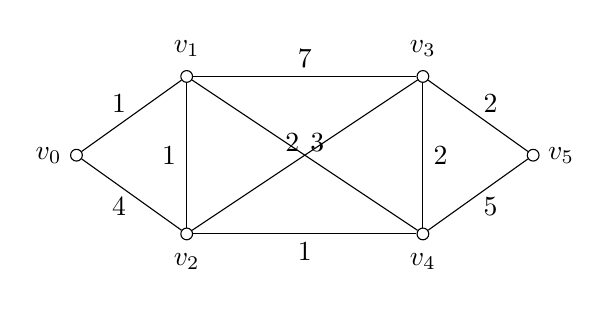
\begin{tikzpicture}[scale=1.0,every node/.style={circle,draw,inner sep=1.5pt}]
        \node[label=left:$v_0$] (v0) at (0,0) {};
        \node[label=above:$v_1$] (v1) at (1.4,1) {};
        \node[label=below:$v_2$] (v2) at (1.4,-1) {};
        \node[label=above:$v_3$] (v3) at (4.4,1) {};
        \node[label=below:$v_4$] (v4) at (4.4,-1) {};
        \node[label=right:$v_5$] (v5) at (5.8,0) {};

        \draw (v0)--node[above left,draw=none]{$1$}(v1);
        \draw (v0)--node[below left,draw=none]{$4$}(v2);
        \draw (v1)--node[left,draw=none]{$1$}(v2);
        \draw (v1)--node[above,draw=none]{$7$}(v3);
        \draw (v2)--node[below,draw=none]{$1$}(v4);
        \draw (v3)--node[right,draw=none]{$2$}(v4);
        \draw (v3)--node[above right,draw=none]{$2$}(v5);
        \draw (v4)--node[below right,draw=none]{$5$}(v5);
        \draw (v1)--node[above right,draw=none]{$3$}(v4);
        \draw (v2)--node[above left,draw=none]{$2$}(v3);
    \end{tikzpicture}
    \end{center}

    \item 在通信中，设八进制数字出现的频率如下：
    \begin{center}
    \begin{tabular}{cccc}
        $0:\ 25\%$ & $1:\ 20\%$ & $2:\ 15\%$ & $3:\ 10\%$ \\
        $4:\ 10\%$ & $5:\ 10\%$ & $6:\ 5\%$ & $7:\ 5\%$
    \end{tabular}
    \end{center}
    采用 $2$ 元前缀码，求传输数字最少的 $2$ 元前缀码，并求传输 $100$ 个按上述比例出现的八进制数字需要多少个二进制数字？若用等长的（长为 $3$）的码字传输需要多少个二进制数字？
\end{enumerate}
